\documentclass{standalone}
\usepackage{mathpazo}
\usepackage[american voltages, american currents]{circuitikz}

\begin{document}
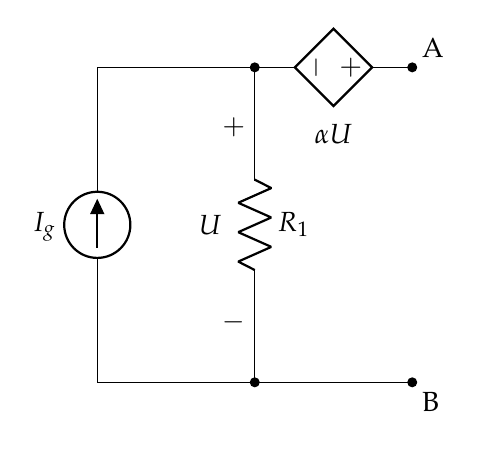
\begin{tikzpicture}
  \coordinate (A) at (0,4);
  \coordinate (B) at (2,4);
  \coordinate (C) at (4,4);
  \coordinate (D) at (0,0);
  \coordinate (E) at (2,0);
  \coordinate (F) at (4,0);
  \draw
  (A) to [short, -*] (B)
  (C) to [cV, *-, v=$\alpha U$] (B)
  (C) node[above right] {A} to [open] (F) node[below right] {B}
  (D) to [short, -*] (E) to [short, -*] (F)
  (D) to [isource, l=$I_g$] (A)
  (B) to [R, l= $R_1$, v=$U$] (E);
  \end{tikzpicture}
\end{document}